\documentclass{article}
\usepackage[utf8]{inputenc}
\usepackage{graphicx}
\usepackage{hyperref}

\title{Systems Analysis \& Design \\ Semester 2025-I \\ Workshop No. 2 — Kaggle Systems Design}
\author{
    Juan David Escallon Guzmán \\
    Juan Diego Lozano Luna \\
    Jorge Eduardo Muñoz Gomez \\
    Universidad Distrital Francisco José de Caldas
}
\date{}

\begin{document}

\maketitle

\section*{Introduction}
In workshop 1, we conduct a systematic analysis of the Kaggle competition "Google Research Football with Manchester City F.C.", where the competitors must create an IA Agent that plays as a team in a football simulation, controlling just one player at time, and playing matches against other competitors' AI agents. During the analysis we thought of the competition as a system, allowing us to characterize all the elements of the competition and the relationships between them, and the critical elements in it that must be considered. In this workshop, we will take what we learned in the first workshop to design our own IA agent that fulfills the competition requirements.

\section*{Review of the Findings from Workshop 1}
During workshop 1, the competition was well described. The open-sourced test environment provided by Google Research will allow us to train and test our AI Agent through simulated football matches. Also provides us with different scenarios like counterattack, or empty goal for this propose. Another thing described is the flow of a match, where the duration of this is given by 3000 turns for the AI Agent to choose an action of the 19 possible based on the environmental information, which is provided to the agent in a variety of formats. Thanks to the analysis done, we determined that the two best formats are raw, which includes all the information possible about the match, and simple115\_v2, which is an observation wrapper that shows the game state based on floats. Every observation wrapper contains information like coordinates and direction of each team player, coordinates and direction of the ball, and the team with the ball, but excludes some information like yellow card per team, or tired factor.

Another thing mentioned was the training model that should be used in this case, being Reinforcement Language (RL) since we were provided with a good simulation environment, being the RL algorithm chosen the Proximal Policy Optimization (PPO) since it displays a more consistent progression compared to other algorithms. We also talk about the different behaviors that are experimented during different stages of a match, and how this could be a factor to take into consideration. Finally, we talk about how chaotic a football match could be, and how this could make the learning process of the AI agent go wrong, something that invites us to think about a backup for the training process.

\section*{System Requirements}
Once we outlined the principal outcomes from Workshop 1, we could determine the requirements that we need to fulfill when develop our AI Agent:

\begin{figure}[htbp]
    \centering
    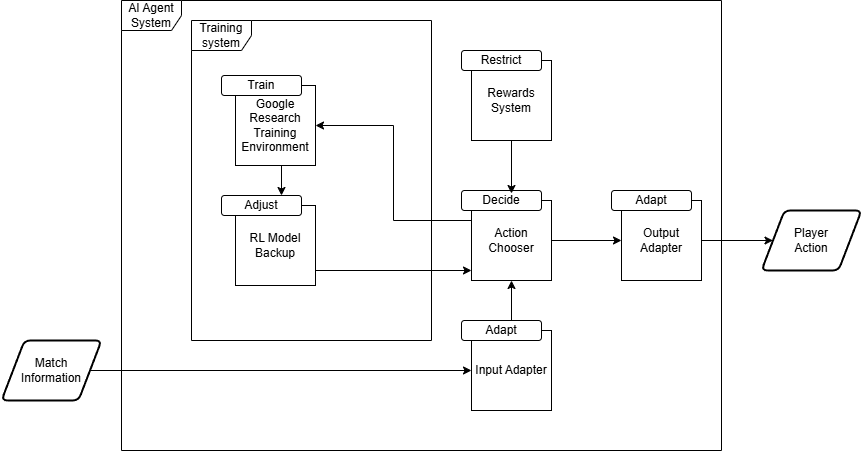
\includegraphics[width=0.9\textwidth]{SystemDiagram.png}
    \caption{Proposed architecture for the AI Agent system.}
    \label{fig:architecture}
\end{figure}

\begin{itemize}
    \item The system must be able to recognize the game information in any format given by the environment.
    \item The system must be able to choose an action for the controlled player, given the information of the game.
    \item The system must be submitted to the competition in the correct format (with the function agent(obs))
    \item The system must be trained to make better decisions when choosing an action during a match.
    \item The system should consider the football and competition rules for the matches. This is achieved by a good reward system modeling.
    \item The system should save different versions of the RL model while training to prevent potential regressions in learning.
\end{itemize}

\section*{System Architecture}
Based on the requirements established on the previous part, we proposed the next architecture for the AI Agent system:

\begin{itemize}
    \item \textbf{Input Adapter:} This component will receive the match information and standardize its format, which will allow us to adapt the system to different the information representations formats mentioned in workshop 1.
    
    \item \textbf{Action Chooser:} This component is where the RL is implemented and will decide the player action based on the information received from the input adapter.
    
    \item \textbf{Rewards System:} This element contains the rules under which the RL model learns. Here are represented things like different behavior in different phases of the match, or restrictions related to the rules.
    
    \item \textbf{Output Adapter:} Receive the action generated by the action chooser and put it in an environment compatible format to be used.
    
    \item \textbf{Google Research Environment:} This is the environment provided by the competition to train our AI agents. It includes different scenarios to train our RL model under different conditions and improve their learning process.
    
    \item \textbf{RL Model Backup:} This is the place where the RL model will be saved every certain number of training stages as a backup plan in chase that the RL model learns something that should. This component will adjust the Action Chooser with the last functional RL model.
\end{itemize}

\section*{Addressing Sensitivity and Chaos}
Talking about the sensitivity, in workshop 1 the format of observation was identified as an element with high sensitivity, so we bring the output adapter as a strategy to increase the adaptability of the system in the same context (football simulation). Elements related to the playing style, or the action set was identified as an element with medium sensitivity in the system, so we considered the rewards system of the RL model as a whole element, so we could modify the values of it and try how it could improve the quality of the decisions. Now talking about the chaos, we implemented the RL Model Backup since we identified how chaotic the environment was, this brings us a secure way to try crazy rewards systems with any fear of lost all our work.

\section*{Technical Stack and Implementation Sketch}
For the implementation of this system, we recommend using python as the main coding language, since it will allow us to use easily the framework TensorFlow, a powerful tool that helps with managing and implementing machine learning processes. The library Agents of TensorFlow facilitates and standardizes the development of Reinforcement Learning, which we already determinate that was necessary to the AI agent. A tool like Docker will let us to use easily the test environment provided by Google Research in its different scenarios since we will be able to make all the Linux-oriented installations required faster. And a tool like GitHub could help us to control the versions of the RL model, as talked in the structure.

Finally, a brief plan on how components could be implemented is given, where the Input Adapter could follow a dictionary structure to standardize the match information to easily have access from the Action Chooser. Talking about the Action Chooser, this is going to implement with help from the already mentioned Agents library, where there is a first version of the rewards system, which change according to the situation of the team, or the role of the controlled player. The first version of the rewards system is structured as low, medium, and high rewards or penalties, and is next specified:

\subsection*{Goalkeeper}
\textbf{Defense:}
\begin{itemize}
    \item Must stay near the goal area. Moving too far from this zone results in a high penalty.
    \item If the ball passes the goal line: very high penalty.
    \item Passing to an opponent: high penalty.
    \item Receiving a yellow card: medium penalty.
    \item Committing a foul inside the box: very high penalty.
\end{itemize}

\textbf{Attack:}
\begin{itemize}
    \item Completing a successful pass: very high reward.
\end{itemize}

\subsection*{Center Back}
\textbf{Defense:}
\begin{itemize}
    \item Ball in their own defensive area: high penalty.
    \item Ball in the opponent's area: high penalty.
    \item Yellow card: medium penalty.
    \item Foul inside the box: very high penalty.
\end{itemize}

\textbf{Attack:}
\begin{itemize}
    \item Successful forward pass: high reward.
    \item Successful backward pass: medium reward.
    \item Failed pass: high penalty.
    \item Scoring a goal: very high reward.
\end{itemize}

\subsection*{Full Back (Wing Back / Lateral)}
\textbf{Defense:}
\begin{itemize}
    \item Ball in their own defensive area: high penalty.
    \item Ball in the opponent's area: high penalty.
    \item Yellow card: medium penalty.
    \item Foul inside the box: very high penalty.
\end{itemize}

\textbf{Attack:}
\begin{itemize}
    \item Successful forward pass: high reward.
    \item Successful backward pass: medium reward.
    \item Failed pass: high penalty.
    \item Scoring a goal: very high reward.
    \item Sprinting down the wings: high reward.
\end{itemize}

\subsection*{Central Midfielder}
\textbf{Defense:}
\begin{itemize}
    \item Ball in their own half: medium penalty.
    \item Ball in the opponent's half: high penalty.
    \item Yellow card: medium penalty.
    \item Foul inside the box: very high penalty.
\end{itemize}

\textbf{Attack:}
\begin{itemize}
    \item Successful forward pass: high reward.
    \item Successful backward pass: medium reward.
    \item Failed pass: high penalty.
    \item Scoring a goal: very high reward.
    \item Sprinting down the wings: high reward.
\end{itemize}

\subsection*{Striker (Center Forward)}
\textbf{Defense:}
\begin{itemize}
    \item Ball in their own half: medium penalty.
    \item Ball in the opponent's half: low penalty.
    \item Staying in their own half: low penalty.
    \item Yellow card: medium penalty.
    \item Foul inside the box: very high penalty.
\end{itemize}

\textbf{Attack:}
\begin{itemize}
    \item Successful forward pass: high reward.
    \item Successful backward pass: medium reward.
    \item Failed pass: high penalty.
    \item Scoring a goal: very high reward.
    \item Sprinting down the wings: high reward.
    \item Taking a shot: high reward.
\end{itemize}

\subsection*{Winger}
\textbf{Defense:}
\begin{itemize}
    \item Ball in their own half: medium penalty.
    \item Ball in the opponent's half: low penalty.
    \item Staying in their own half: low penalty.
    \item Yellow card: medium penalty.
    \item Foul inside the box: very high penalty.
\end{itemize}

\textbf{Attack:}
\begin{itemize}
    \item Successful forward pass: high reward.
    \item Successful backward pass: medium reward.
    \item Failed pass: high penalty.
    \item Scoring a goal: very high reward.
    \item Sprinting down the wings: high reward.
    \item Successful cross into the box: high reward.
\end{itemize}

The Output Adapter is going to be a class with the method agent(obs), in this method is where the elements are integrated, since we are going to standardize the input observations to give it to the Action Chooser, which will give the player action based on the RL model, and its returned to the environment in a compatible format.

\section*{Bibliography}
\begin{itemize}
    \item TensorFlow. (n.d.). TF-Agents: A reliable, scalable, and easy-to-use TensorFlow library for Reinforcement Learning. \url{https://www.tensorflow.org/agents?hl=es-419}
    \item Escallon Guzmán, J. D., Lozano Luna, J. D., \& Muñoz Gomez, J. E. (2025). Workshop No. 1 — Kaggle Systems Engineering Analysis [Workshop report]. GitHub. \url{https://github.com/judlozanol/Systems-Analysis/tree/main/workshop1}
\end{itemize}

\end{document}